\input{header_slides.tex}

\begin{document}

\title{Modelling growth of urban firm networks}
\author{J.~Raimbault$^{1,2,3,4,\ast}$ \and N. Zdanowska$^{5,2,4}$ \and E. Arcaute$^{2}$\\
$\ast$\texttt{juste.raimbault@ign.fr}
}

\institute{$^{1}$LASTIG, Univ Gustave Eiffel, IGN-ENSG\\
$^{2}$CASA, UCL\\
$^{3}$UPS CNRS 3611 ISC-PIF\\
$^{4}$UMR CNRS 8504 G{\'e}ographie-cit{\'e}s\\
$^{5}$Luxembourg Institute of Socio-Economic Research
}




\date{CCS 2022\\
UrbanSys Satellite\\
19/10/2022
}

\frame{\maketitle}


% extended abstract
% The emergence of interconnected urban networks is a crucial feature of globalisation processes. Understanding the drivers behind the growth of such networks – in particular urban firm networks –, is essential for the economic resilience of urban systems. We introduce in this paper a generative model for firm networks at the urban area level, which considers the following features: the economic size of the areas representing the source and target nodes, the industrial sector proximity between firms, the strength of links from the past, as well as the geographical and socio-cultural distances between urban areas. These are combined into a generalised spatial interaction model giving the probability to add links between urban areas, used in an iterative manner to generate the network from an initial configuration.
%An empirical network analysis on European urban firm ownership data confirms the relevance of each of these factors on new link creation. We construct a directed network between functional urban areas in Europe, based on the AMADEUS data which is a well covering dataset describing ownership links between companies and their subsidiaries. The links between firms are aggregated at the urban area level and economic size of areas are computed by aggregating turnovers of firms. A community detection analysis provides a community structure which is partly geographical but also captures some known economic collaboration areas (see Fig. 1). Statistical models (various specifications of spatial interaction models) assess the role of various factors to be included in the simulation model.
%We then simulate network growth on synthetic systems of cities with the generative model. Examples of generated networks are shown in Fig. 1. Global sensitivity analysis provides the influence of parameters on model outputs characterising network structure. A grid sampling of the parameter space unveils stylised facts such as a transition from a local to a global regime or a maximal integration achieved at an intermediate interaction range.
%We calibrate the model on the European network, with a real geographical setup and economic sector composition obtained from the empirical network data. Calibration is done on two objectives, in order to reproduce the real network in terms of link weights (mean squared error on weights and mean squared error on logarithms of weights), with a genetic algorithm for bi-objective optimisation (NSGA2). Considering the common fitting objective, the simulation model outperforms statistical models. This furthermore shows a strong role of path-dependency for model performance.
%The model is finally applied to stylised scenarios, where economic shocks modify spatial interaction parameters after a fixed number of time steps. This opens up to the formulation of public policies recommendations to deal with exogenous shocks such as economic crises or potential lock-downs of countries.
% Fig 2, 3
% Figure 1: (Left) Empirical analysis of the AMADEUS data: urban area size corresponds to economic size, while color gives the community obtained with a Louvain modularity optimisation algorithm; (Right) Example of simulated networks: top row in a synthetic system with long-range interactions (left) and short range interactions (right), bottom row with same parameter values but in the real setting.






\section{Introduction}


\sframe{Urban firm networks}{


%General framework:
\textit{Role of firm networks in urban systems:}

\medskip

\begin{itemize}
\item Cities as cross-overs of socio-economic interactions           \cite{castells1996information}
    \item Networks as the new social morphology of societies \cite{castells2000networksociety}, giving rise to network economies \cite{sassen1991global} 
    \item Emergence of an interconnected world city network as a crucial feature of globalisation \cite{taylor2001specification}  
    \item Interurban interactions between firms as one of the most representative of economic trends \cite{martinus2018global}
    
\end{itemize}

\bigskip

}

\sframe{An evolutionary approach to Urban Systems}{


\textit{Relevance of dynamics urban network evolution models:}

\medskip

\begin{itemize}
    \item Evolutionary Theory of Urban Systems \cite{pumain1997pour} \cite{pumain2006villes}
    \item Adaptive cycles and diffusion of innovation \cite{Hagerstrand1968Innovation}
    \item Path dependence \cite{martin2006path} \cite{pumain2012urban}
    \item Selection and emerging structures of systems 
    \item Evolutionary models for urban systems dynamics: \cite{favaro2011gibrat} \cite{cottineau2015growing} \cite{schmitt2015half} \cite{raimbault2018calibration} \cite{raimbault2018indirect} \cite{Raimbault_2020}
\end{itemize}

}

\sframe{Urban firm linkages and geo-economic processes}{

Main geographical processes considered:

\medskip

\begin{itemize}
    \item Metropolisation \& internationalisation effects
    \item Specialisation-driven factors and drivers of innovation
    \item Macroeconomic exogenous chocs and resilience of urban systems 
\end{itemize}

\bigskip

$\rightarrow$ \textit{How can we capture geographical and economic processes within urban networks of firms with a generative model?}

\medskip

Advantages of the model introduced:

\medskip

\begin{itemize}
	\item Indirect inference on processes
	\item Multiple complementary factors driving inter-urban links
	\item Includes path-dependency
\end{itemize}

}

\sframe{Contribution}{

We examine the interactions of European cities within firm linkages defined by
corporate ownership links and introduce

\medskip

\begin{itemize}
    \item an empirical analysis of the firm ownership urban network in the European Union, based on the Bureau Van Dijk's AMADEUS database;
    \item a generative network model to simulate the growth of such linkages at urban areas scale;
    \item the model allows us to compare the effect of different factors on the final network structure, which is extensively studied through model sensitivity analysis and exploration;
   \item we calibrate the model on the empirical network and apply it to stylized economic shock scenarios.
\end{itemize}

}

\section{Model}

\sframe{Model rationale}{

$\rightarrow$ Cities are defined by their GDP and their profile regarding the proportion of firms in the different sectors. Links between cities are created in an iterative way, taking into account:

\medskip

    \begin{itemize}
        \item geographical proximity (distance or effective accessibility)
        \item geopolitical proximity (belonging to the same country or single market $\rightarrow$ application to Brexit)
        \item city size (economic size as GDP) 
        \item economic similarity (e.g. cosine distance between sector proximity as done in \cite{2019arXiv190505106C}
        \item previous linkages 
    \end{itemize}

}


\sframe{Formalization}{

Cities characterised by economic size $E_i$ (GDP) and economic structure $S_{ik}$ (probability distribution of firms within $K$ sectors)


\medskip

Starting from an initial network, at each time step, add a fixed number of links randomly, following a probability as a generalised Cobb-Douglas function

\[
     p_{ij} \propto \left(\frac{E_{i}}{E}\right)^{\gamma_O} \cdot \left(\frac{E_{j}}{E}\right)^{\gamma_D} \cdot \left(\frac{w_{ij}}{W}\right)^{\gamma_W} \cdot s\left(S_{ik},S_{jk}\right)^{\gamma_S} \cdot \exp \left(- \frac{d_{ij}}{ d_0}\right) \cdot \exp \left(- \frac{c_{ij}}{c_0}\right)
\]

where $E \textrm{ = } \sum_k E_k$, $W \textrm{ = } \sum_{i,j} w_{ij}$, $s$ is a proximity measure given by cosine similarity, $d_{ij}$ euclidian distance, and $c_{ij}$ a socio-cultural distance

\medskip

\textbf{Model parameters: } $\gamma_O, \gamma_D, \gamma_W, \gamma_S, d_0, c_0$

\medskip

\textbf{Model indicators: } internationalisation (modularity of countries in the network), metropolisation (correlation between weighted degree and city size), optimal modularity, average community size

}


\sframe{Empirical data}{

 \begin{center}
 \includegraphics[width=0.7\textwidth]{../../figures/Fig2.png}
 \end{center}
 
 \footnotesize
 
  \textit{Map of network communities obtained by modularity maximisation (European ownership network between Functional Urban Areas, constructed from the AMADEUS database).}

}



\sframe{Empirical network properties}{

\begin{center}
    \includegraphics[width=\linewidth]{../../figures/Fig1.png}
\end{center}

\textit{Empirical distribution of network properties, with log-normal and power law fits}

}


\begin{frame}[label=statmain]

\frametitle{Statistical models}



Most general spatial interaction model with fixed effects:

\begin{equation}
\log w_{ij} \textrm{ = } \log d_{ij} \textrm{ + } \log T_i \textrm{ + } \log T_j \textrm{ + } \log s_{ij} \textrm{ + } \alpha_{c_i,c_j} \textrm{ + } \varepsilon_{ij}
\end{equation}

\bigskip
\bigskip

\resizebox{\linewidth}{!}{
\begin{tabular}{|l|c|c|c|c|c|c|c|c|c|c|c|c|}
\hline
 & \multicolumn{2}{|c|}{$d_0$} & \multicolumn{2}{|c|}{$c_0$} & \multicolumn{2}{|c|}{$\gamma_S$} & \multicolumn{2}{|c|}{$\gamma_W$} & \multicolumn{2}{|c|}{$\gamma_O$} & \multicolumn{2}{|c|}{$\gamma_D$} \\
 & F & T & F & T & F & T & F & T & F & T & F & T \\
 \hline
Internationalisation & 0.2 & 0.3 & 0.7 & 0.7 & 0.001 & 0.008 & $5\cdot 10^{-4}$ & 0.007 & 0.03 & 0.04 & 0.02 & 0.04 \\
Metropolisation & 0.02 & 0.04 & 0.02 & 0.04 & 0.02 & 0.3 & 0.002 & 0.01 & 0.2 & 0.7 & 0.2 & 0.7 \\
Modularity & 0.3 & 0.4 & 0.6 & 0.6 & $5\cdot 10^{-4}$ & 0.02 & 0.002 & 0.02 & 0.007 & 0.03 & 0.003 & 0.03 \\
Avg. com. size & 0.004 & 0.1 & 0.01 & 0.1 & 0.003 & 0.07 & 0.001 & 0.04 & 0.3 & 0.6 & 0.3 & 0.6 \\
Degree entropy & 0.003 & 0.03 & 0.002 & 0.03 & 0.008 & 0.04 & 0.003 & 0.03 & 0.5 & 0.6 & 0.5 & 0.6 \\
Weight entropy & 0.04 & 0.2 & 0.03 & 0.2 & 0.002 & 0.1 & 0.001 & 0.1 & 0.5 & 0.6 & 0.5 & 0.6 \\\hline
\end{tabular}
}

\bigskip

Zero-inflated and Hurdle models: \hyperlink{zeroinfl}{\beamerbutton{Details}}

\end{frame}




\begin{frame}[label=setupmain]

\frametitle{Model setup}

\justify
 
\begin{enumerate} 
    \item Simulation on synthetic systems of cities \cite{raimbault2019space}: generation of a continent-scale urban system with stylized order of magnitude corresponding to Europe (urban hierarchy, countries, industrial sector distributions - \hyperlink{syntheticsetup}{\beamerbutton{Details}})
    \bigskip
    \item Simulation on the European system of cities, setup with AMADEUS data at FUA level (\hyperlink{realsetup}{\beamerbutton{Details}})
\end{enumerate}

\end{frame}


\section{Results}

\sframe{Implementation and experiments}{

\footnotesize

\textbf{Implementation}

\begin{itemize}
	\item Model implemented in NetLogo (good compromise interactivity / ergonomy), with fast data structures (matrix/table extensions)
	\item Integrated seamlessly into OpenMOLE \cite{reuillon2013openmole} for model exploration \url{https://openmole.org/}
\end{itemize}

\begin{center}
\includegraphics[width=0.1\linewidth]{../../figuresraw/iconOM.png}
\includegraphics[width=0.4\linewidth]{../../figuresraw/openmole.png}
\end{center}

\medskip

\textbf{Experiments}

\begin{itemize}
	\item One-factor sampling with 100 repetitions to assess statistical properties (good convergence, average sharpe ratios for indicators all larger than 5)
	\item Grid sampling with 20 repetitions for model behavior
	\item Targeted experiment on impact of synthetic hierarchy
	\item Global Sensitivity Analysis \cite{saltelli2008global}
	\item Calibration on real setup with a Genetic Algorithm
	\item Application to economic shocks scenarios
\end{itemize}

}

\sframe{Simulation of urban networks}{


 \begin{center}
 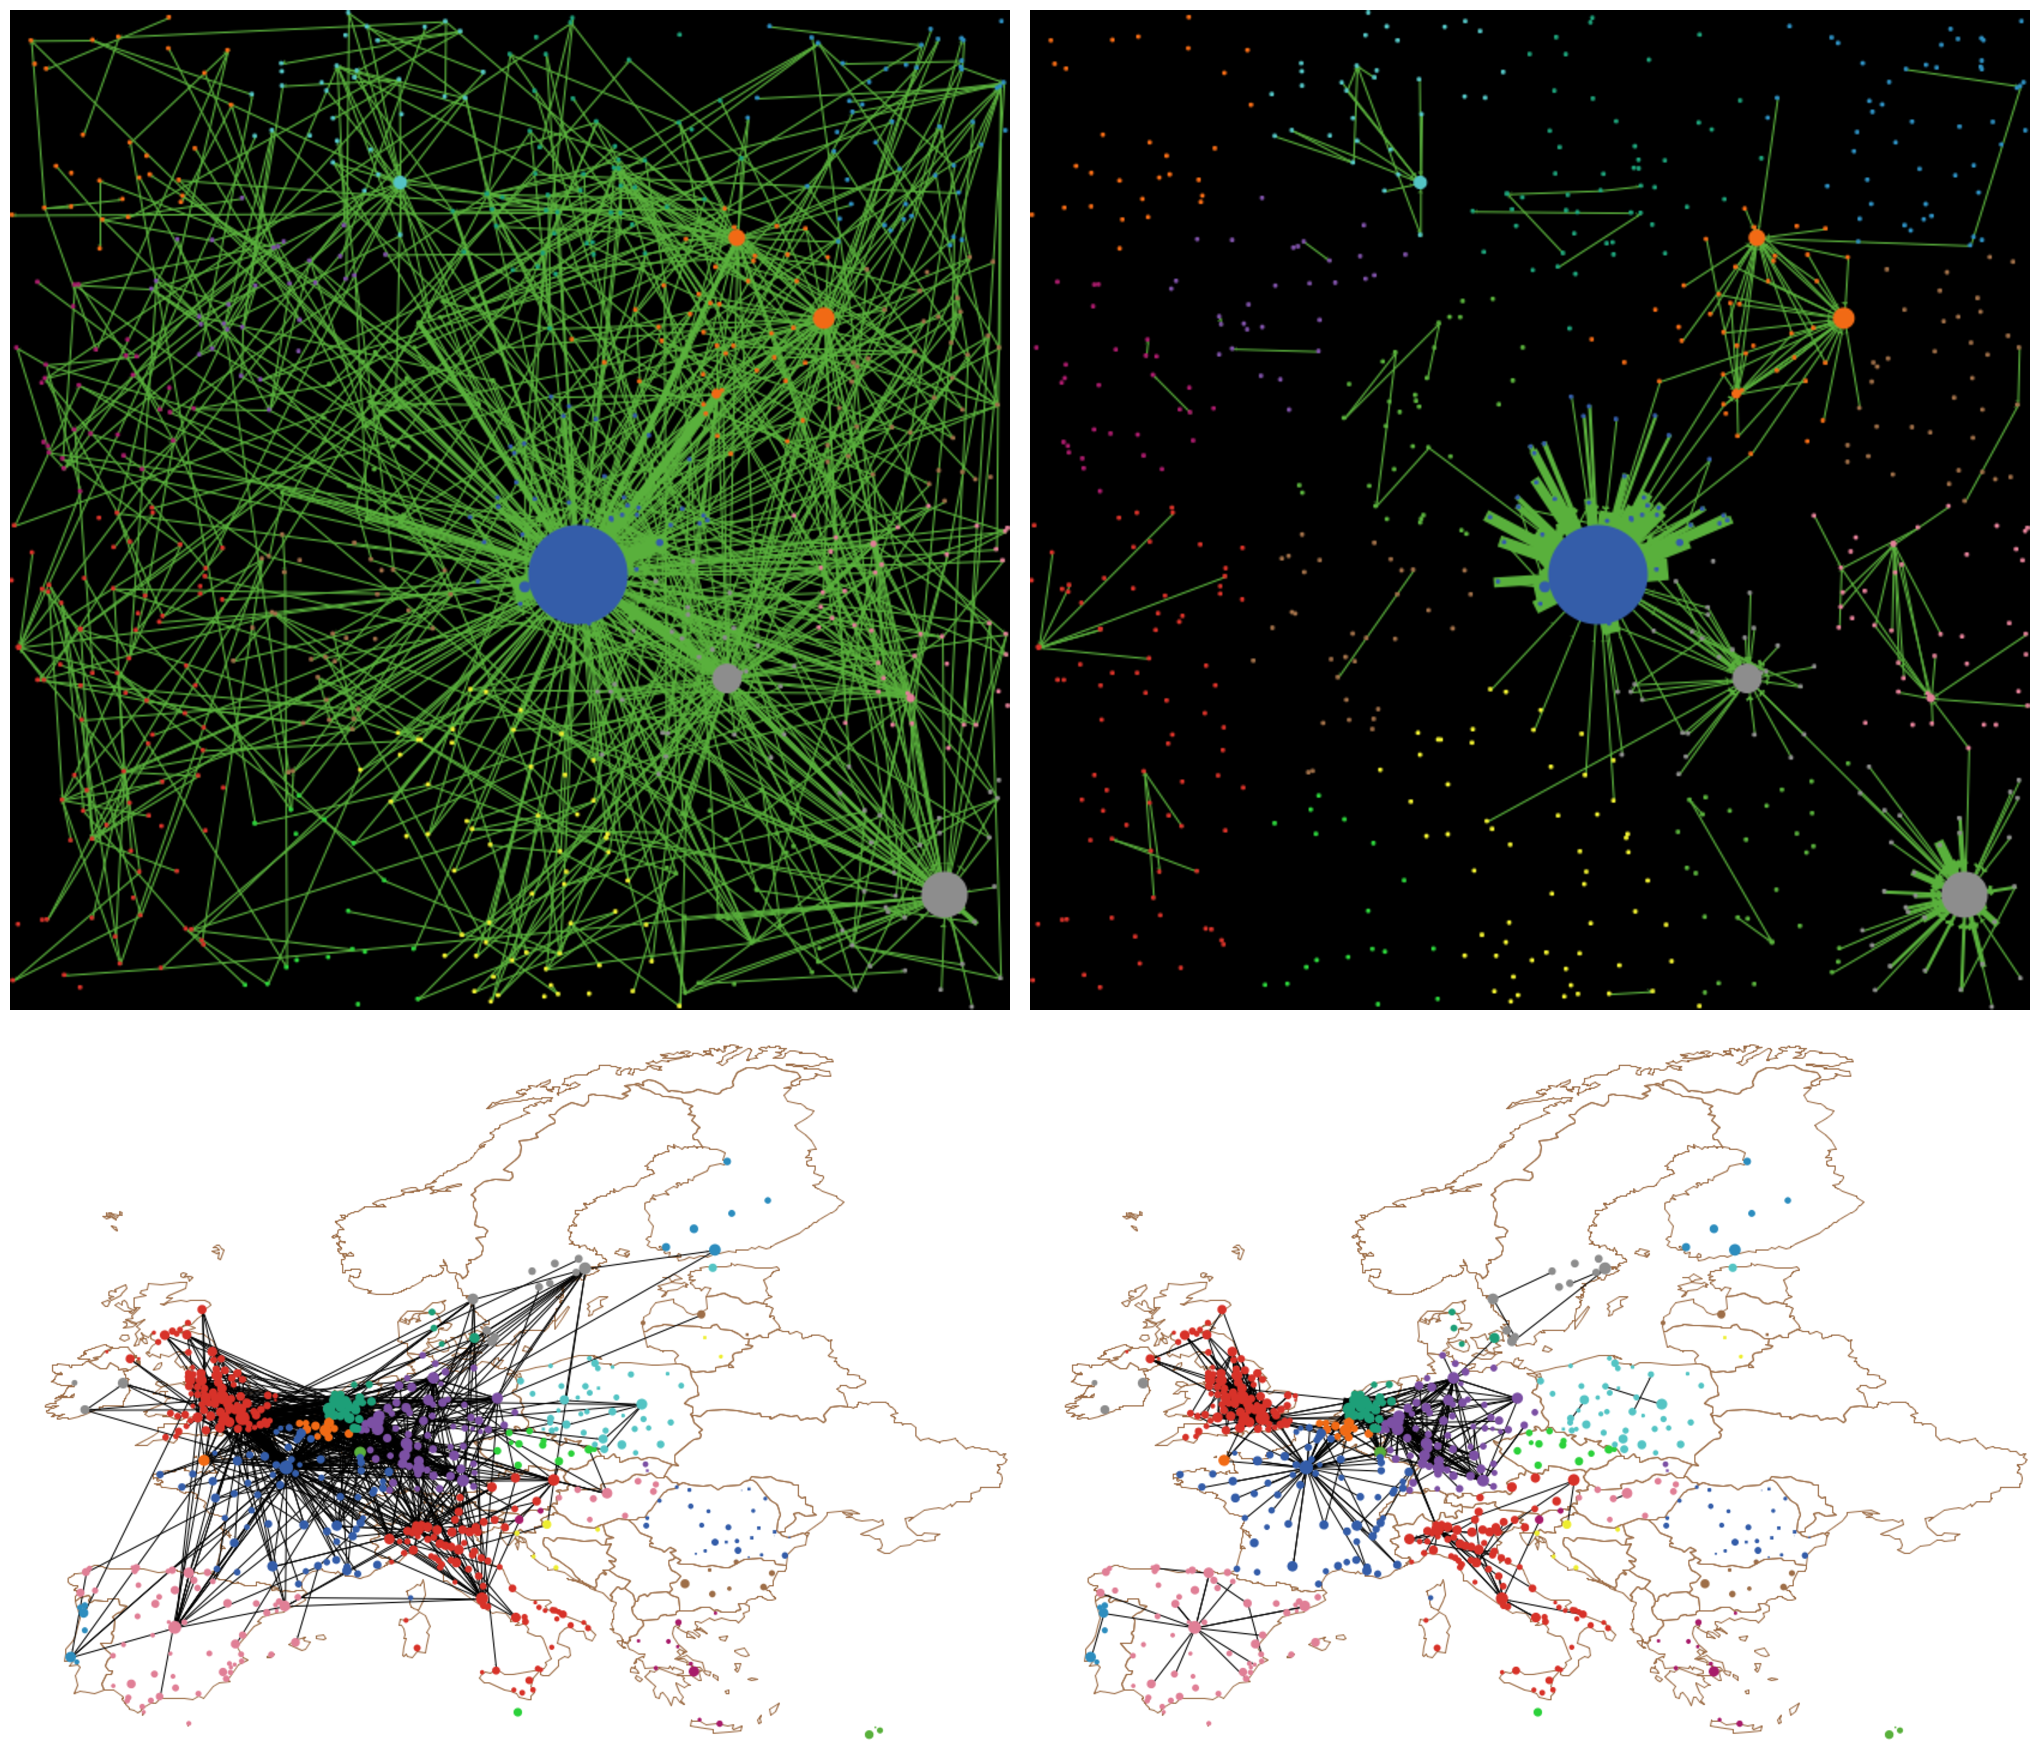
\includegraphics[width=0.67\textwidth]{../../figures/Fig3.png}
 \end{center}

\footnotesize

	\textit{Simulated networks in a synthetic setup (top) and real setup (bottom), for a large (resp. low) interaction range $d_0$ (left, resp. right).}

}


\sframe{Effect of interaction decay}{
    
    \includegraphics[width=0.48\textwidth]{../../figuresraw/internationalisation-gravityDecay_errorbars.png}
    \includegraphics[width=0.48\textwidth]{../../figuresraw/metropolisation-gravityDecay_errorbars.png}
    
    \medskip
    
    \footnotesize
    
    \textit{(Left) Internationalisation index decreases exponentially with gravity decay; (Right) metropolisation also shows a progressive transition from a local to a global regime.}
    
}


\sframe{Effect of sector proximity}{
    
     \includegraphics[width=0.48\textwidth]{../../figuresraw/internationalisation-gammaSectors_errorbars.png}
    \includegraphics[width=0.48\textwidth]{../../figuresraw/metropolisation-gammaSectors_errorbars.png}
    
    \medskip
    \footnotesize
    
    \textit{(Left) Internationalisation varies linearly with sector proximity $\gamma_S$; (Right) metropolisation witnesses an intermediate regime where size is the most important}
        
}

\sframe{Grid exploration: internationalisation}{

     \begin{center}
     \includegraphics[width=\textwidth]{../../figures/Fig5.png}
     \end{center}
     
     \medskip
    
     \footnotesize
    
     \textit{The transition as a function of interaction range depends on the influence of origin size $\gamma_F$; sector proximity $\gamma_S$ plays a role only for a large influence of the origin.}
    
}

\sframe{Grid exploration: community size}{

    \begin{center}
    	\includegraphics[height=0.6\textheight]{../../figures/Fig6.png}
    	
    \end{center}
    
    \vspace{-0.5cm}
    
    \footnotesize

\begin{itemize}
	\item Maximal integration in term of community size is achieved at an intermediate value of $d_G$: emergence of a regional regime
	\item Maximal size depends on the role of sectors $\gamma_S$, in a decreasing way when origin size is deactivated, and increasing way when $\gamma_F=1$
	\item This regime disappear when origin size influence is too large
\end{itemize}
    
}

\sframe{Role of urban hierarchy}{

\begin{center}
    \includegraphics[width=\linewidth]{../../figures/Fig7.png}
\end{center}

\medskip

\textit{Impact of urban hierarchy on model indicators in synthetic systems of cities: existence of a maximum for metropolisation at intermediate hierarchies.}

}


\begin{frame}[label=calibmain]

\frametitle{Calibration on the European urban network}

    \begin{center}
    	\includegraphics[height=0.7\textheight]{../../figures/Fig8.png}
    	
    \end{center}
    
    \footnotesize
    
\textit{Pareto front obtained for the bi-objective model calibration using a NSGA2 algorithm (outperforms statistical models that have a MSE of 5.33).}

    
    % weird point out of pareto front: ?
    
   \hyperlink{calibration}{\beamerbutton{Details}} on the calibration procedure
    
    
    
    
\end{frame}


\sframe{Economic shock scenarios}{

    \begin{center}
    	\includegraphics[height=0.72\textheight]{../../figures/Fig9.png}
    	
    \end{center}
    
    %\vspace{-0.5cm}
    
    \footnotesize

\textit{Although the system is resilient to moderate shocks, strong restrictions have an important impact on internationalisation and thus can be
expected to have a detrimental effect on UK economy due to these foreign ownership links.}
    
}


\section{Discussion}

\sframe{Discussion}{

\justify

\textbf{Practical applications}

\medskip

$\rightarrow$ Potential application to public policy issues;

\medskip

$\rightarrow$ Effect of exogenous shocks on specific economic sectors mostly dependent on foreign ownership links (extraction of crude petroleum, manufacture of tobacco \& basic pharmaceutical goods, activities of head offices).

\bigskip
\bigskip

\textbf{Developments}

\medskip

$\rightarrow$ co-evolution model (evolution of city sizes) \cite{raimbault2021modeling};

\medskip

$\rightarrow$ a model with firm agents (multi-scale ABM) \cite{raimbault:halshs-02351722};

\medskip

$\rightarrow$ targeted study of path dependency;

\medskip

$\rightarrow$ other formulation of the combination of factors or multi-objective optimisation depending on sectors using Pareto fronts.


}


\sframe{Conclusion}{

$\rightarrow$ A generative model to understand processes of economic network emergence

\bigskip

$\rightarrow$ Crucial role of model exploration to validate and extract knowledge from such a simulation model


\bigskip
\bigskip

\textbf{Preprint at} \texttt{https://arxiv.org/abs/2009.05528}

\bigskip

\textbf{Open repository for model and results at}

\texttt{https://github.com/JusteRaimbault/ABMCitiesFirms}

\bigskip

\textbf{Simulation data at} \texttt{https://doi.org/10.7910/DVN/UPX23S}

\bigskip

\textbf{Acknowledgments}: thanks to the \textit{European Grid Infrastructure} for access to the infrastructure. We also acknowledge the funding of the EPSRC grant EP/M023583/1


}



%%%%%%%%%%%%%%%%%%%%%
\begin{frame}[allowframebreaks]
\frametitle{References}
\bibliographystyle{apalike}
\bibliography{biblio}
\end{frame}
%%%%%%%%%%%%%%%%%%%%%%%%%%%%




\sframe{Reserve slides}{

\Huge

\centering

Reserve slides

}



\begin{frame}[label=syntheticsetup]

\frametitle{Synthetic setup}

\begin{enumerate}
    \item Generate $N \textrm{ = } 700$ cities with size following a power law $E_i \textrm{ = } E_0 \cdot i^{-\alpha}$ with $E_0 \textrm{ = } 10^{11}$ and $\alpha \textrm{ = } 1.1$ (computed on Europe for GDP with cities larger than 50.000 inhabitants)
    \item Distribute them randomly in space (\cite{simini2019testing} vs \cite{banos2011christaller})
    \item Create countries with k-means clustering ($C \textrm{ = } 30$)
    \item Distribute sectors such that (i) smaller cities are more specialised and (ii) larger cities are more knowledge-based, with a one dimensional axis to position sectors $1/K \ldots 1$ where the density $f\left(k\right)$ follows a log-normal with $\left(\mu,\sigma\right)$ such that $\sqrt{\Var f} \textrm{ = } K/2$ for the largest, $\sqrt{\Var f} \textrm{ = } 1/K$ for the smallest % equations? too much -> refer to paper
\end{enumerate}

\hyperlink{setupmain}{\beamerbutton{Back}}

\end{frame}



\begin{frame}[label=realsetup]

\frametitle{Real configuration setup}

% sociocultural distance

Urban areas (FUAs) positions, economic size initialised from the GHSL database, sector composition from the Amadeus database using classification of firms and aggregating

\bigskip

Initial dummy network ($w_0 = 1$)

\bigskip

\textbf{Socio-cultural distance} $c_{ij}$: fixed effects coefficients

% Q: how are NAs handled?: infinite: ~ - anyway not used in calibration

\begin{tabular}{ccccccc}
   Min. & 1st Qu. &  Median &  Mean &  3rd Qu. &  Max. &  NA's \\
 -2.327 &  1.440 &  2.451 &  2.538 &  3.447 & 11.797 &  339 
\end{tabular}

\hyperlink{setupmain}{\beamerbutton{Back}}

\end{frame}



\sframe{Global sensitivity analysis}{


\begin{center}
\resizebox{\linewidth}{!}{
    \begin{tabular}{|l|c|c|c|c|c|c|c|c|c|c|c|c|}
\hline
 & \multicolumn{2}{|c|}{$d_0$} & \multicolumn{2}{|c|}{$c_0$} & \multicolumn{2}{|c|}{$\gamma_S$} & \multicolumn{2}{|c|}{$\gamma_W$} & \multicolumn{2}{|c|}{$\gamma_O$} & \multicolumn{2}{|c|}{$\gamma_D$} \\
 & F & T & F & T & F & T & F & T & F & T & F & T \\
 \hline
Internationalisation & 0.2 & 0.3 & 0.7 & 0.7 & 0.001 & 0.009 & $4\cdot 10^{-4}$ & 0.007 & 0.03 & 0.04 & 0.02 & 0.04 \\
Metropolisation & 0.02 & 0.1 & 0.02 & 0.2 & 0.002 & 0.1 & 0.001 & 0.09 & 0.2 & 0.6 & 0.3 & 0.6 \\
Modularity & 0.3 & 0.4 & 0.6 & 0.6 & 0.004 & 0.02 & $3\cdot 10^{-4}$ & 0.01 & 0.005 & 0.03 & 0.002 & 0.03 \\
Avg. com. size & 0.008 & 0.09 & 0.01 & 0.1 & 0.002 & 0.07 & 0.003 & 0.04 & 0.3 & 0.6 & 0.4 & 0.6 \\
Degree entropy & 0.006 & 0.02 & 0.003 & 0.02 & 0.006 & 0.03 & 0.008 & 0.02 & 0.5 & 0.5 & 0.5 & 0.5 \\
Weight entropy & 0.04 & 0.1 & 0.03 & 0.1 & 0.008 & 0.08 & 0.01 & 0.07 & 0.4 & 0.5 & 0.4 & 0.5 \\\hline
\end{tabular}
}
\end{center}

\medskip

\textit{First order and total sensitivity indices \cite{saltelli2010variance}, for all parameters and indicators.}

}




\begin{frame}[label=zeroinfl]

\frametitle{Zero-inflated and Hurdle statistical models}

Accounting for zeros with specific models: same qualitative results

\bigskip

\begin{center}
\resizebox{\linewidth}{!}{
\begin{tabular}{|l|c|c|c|c|}
\hline
Model  & \multicolumn{2}{|c|}{Zero-inflated} & \multicolumn{2}{|c|}{Hurdle} \\ 
 & Count & Zero-infl. & Count & Zero-hurdle \\
\hline
$\log(d_{ij})$ &    -0.28*** (7e-4) &   0.88*** (0.01)      &   -0.29*** (8e-6)   &  -0.75*** (0.01)    \\
$\log(T_i)$ & 0.74*** (4e-6)  & -0.74*** (7e-3)       &   0.74***  (5e-6)     &  0.67*** (5e-3)   \\
$\log(T_j)$ & 0.64*** (4e-6)  & -0.52*** (7e-3)      &    0.64***  (4e-6)     &  0.48*** (5e-3)    \\
$\log(s_{ij})$ & 0.46*** (2e-5)   &  -0.33*** (3e-2)  &  0.45*** (2e-5)       &  0.27*** (0.02)    \\
\hline
$R^2$ &   \multicolumn{2}{|c|}{0.1607}     &  \multicolumn{2}{|c|}{0.1661}  \\
%MSE & & \\
AIC &     \multicolumn{2}{|c|}{5.85e10}    &   \multicolumn{2}{|c|}{5.85e10}  \\
\hline
\end{tabular}
}
\end{center}



\hyperlink{statmain}{\beamerbutton{Back}}

\end{frame}


\begin{frame}[label=calibration]

\frametitle{Model calibration}

\footnotesize

\textbf{To avoid overfitting:} $c_0 = 0$ to deactivate the mechanism

\bigskip

\textbf{Calibration objectives:}

\[
\varepsilon_L = \frac{1}{N^2} \sum_{i,j} \left(\log w_{ij} - \log \hat{w}_{ij} \right)^2
\]

\[
\varepsilon_M = \log\left(\frac{1}{N^2} \sum_{i,j} \left(w_{ij} - \hat{w}_{ij}\right)^2 \right)
\]

\bigskip

\textbf{On macro indicators?} Too much solutions, equifinality

\bigskip

\textbf{Rescale flows:} $w_0$ is arbitrary, so is optimised with rescaling:

\[
\varepsilon_L (k_0) = \frac{1}{N^2} \sum_{i,j} \left(\log w_{ij} - \log \left(k_0 \cdot \hat{w}_{ij} \right) \right)^2
\]

what yields

\[
k_0 = \exp \left[\frac{1}{N^2} \sum_{i,j} \log w_{ij} - \frac{1}{N^2} \sum_{i,j} \log \hat{w}_{ij} \right]
\]



\hyperlink{calibmain}{\beamerbutton{Back}}

\end{frame}









\end{document}

